\documentclass[12pt,a4,english,finnish,pdflatex%,handout
]{beamer}
\definecolor{MyGreen}{RGB}{50, 120, 50}
\usecolortheme[named=MyGreen]{structure}

\usepackage{babel}
\usepackage[utf8]{inputenc}
\usepackage[T1]{fontenc}
\usepackage{amsmath,amssymb} 
\usepackage{animate}
\usepackage{multimedia}

\usepackage{natbib}
\bibpunct[: ]{(}{)}{,}{}{}{;}

\usepackage{tikz}

\usepackage{tipa}

\usepackage{hyperref}

\setbeamertemplate{navigation symbols}{}

\graphicspath{{figures/}}

\setlength{\leftmargini}{0pt}
\setlength{\leftmarginii}{1em}

\newcommand{\kommentti}[1]{
  {\bf[#1]}
}



\begin{document}
\title{Kielen lainaamisen peruskurssi \\
\&\\
Ideoita ((epä)todelliseen) puheeseen} 
\author{Pertti Palo} 
\date{30.7.2023}

\frame{\titlepage
} 

\frame{\frametitle{Land acknowledgement}
We wish to acknowledge and honor the Miami, Delaware, Potawatomi, Kickapoo, and
Shawnee people, on whose ancestral homelands I have worked on this presentation.
}

\frame{\frametitle{Sisällöstä}
  \begin{itemize}
  \item Ollaan Ropeconissa joten lähtökohtaisesti käyttäydytään ihmisiksi ja
  pidetään tämä tila turvallisena.
  \item Peruskurssissa puhutaan jonkin verran kolonalisaatiosta ja sen
  seurauksista, ihmisryhmien alistamisesta, haukkumasanoista jne.
  \item Työpajassa voi vastaavaa sisältöä tulla vastaan, jos se nousee
  keskustelussa esille, mutta materiaaleisani sitä ei ole. 
  \end{itemize}  
}

\frame{\frametitle{Muuta käytännönpuolta}
  \begin{itemize}
    \item Kysyä saa koska vaan.
    \item Jos ette kysele riittävästi kesken esityksen, ensimmäisen 45 minuutin
    lopussa on aikaa kysymyksille ja keskustelulle.
    \item Vaikka tämä ensimmäinen osa onkin esitelmä tarkoitus ei ole, että
    olisin yksin äänessä.
  \end{itemize}
}


\frame{\frametitle{Mitä tuleman pitää?}
  \begin{itemize}
  \item Osa I: Kielen lainaamisen peruskurrssi
    \begin{itemize}
    \item Sisältö ja käytäntö
    \item Tämä dia
    \item Kuka olen ja miksi olen tässä?
    \item Esimerkkitapaus: Announin maailma
    \item Alustavia ajatuksia kielten valinnasta
    \item Pari asiaa kielisukupuista
    \item Keskustelu, jos se ei tapahtunut esityksen aikana
    \end{itemize}
  \item {\usebeamercolor[gray]{} Osa II: Ideoita ((epä)todelliseen) puheeseen}
  \begin{itemize}
    \item  {\usebeamercolor[gray]{} Lohikäärmeiden puheesta!}
    \item  {\usebeamercolor[gray]{} Lintuihmisiä!}
    \item  {\usebeamercolor[gray]{} Puhe ja taikuus!}
    \item  {\usebeamercolor[gray]{} Pääsette miettimään asiaa itse, koska tämä osa on työpaja.}
  \end{itemize}
  \end{itemize}
}

\frame{\frametitle{Kuka mää oon?}
  \begin{columns}
    \begin{column}{5cm}
      \includegraphics[width=\columnwidth]{uti_eva.png}
    \end{column}
    \begin{column}{5cm}
      \begin{itemize}
      \item Pertti Palo
      \item Minulla on pari tutkintoa (löysästi määriteltynä) insinööritieteistä.
      \item Viimeisimpänä olen saanut fonetiikan tohtorin paperin.
      \item Minulla ei ole mitään muodollista pätevyyttä kielenlainaamisen,
      mutta tiedän paljon puheentuotosta ja\ldots
      \end{itemize}
    \end{column}
  \end{columns}
} 

\frame{\frametitle{Jotain taustaa tietysti on}
\begin{itemize}
  \item En ole tekstiin keskittyvä kielitieteilijä vaan puheentutkija ja foneetiikko.
  \item Tänään lähes joka kerta kun käytän sanaa 'kieli' tarkoitan puhuttua
  kieltä - tosin toisinaan tarkoitan anatomian osaa. 
  \item Puheentutkija olen ollut yli 20 vuotta ja ropellusnörtti yli 30 vuotta. 
  \item Viime vuosina olen opetellut suullista tarinankerrontaa, jolla on
  mielenkiintoisia yhteyksiä sekä roolipeleihin että tieteeseen.
\end{itemize}
}


\frame{\frametitle{Mikä minut tänne toi?}

\begin{itemize}
  \item Kaikki alkoi siitä kun sain päähäni että D\&D kaipaa 'hieman' viilausta. 
  \item Ei, ei nykyinen versio (josta en tiedä juuri mitään) vaan suomekielinen 1980-luvun laitos. 
  \item Hyllyyn oli kertynyt myös nippu Maguksia (lehtiä), joiden seikkailuista
  halusin yhdistellä pitkän kampanjan, mutta en käyttää maailmana mitään Known
  World:iä\ldots 
\end{itemize}

}
\frame{\frametitle{Announ -- minun maailmani ja multiversumini}

\begin{itemize}
  \item Alunperin Announ kasvoi kampanjan ympärille.
  \item Myöhemmin ideoita tuli kerättyä world building spostilistalta (90-luku,
  moi), Loren J. Millerin MythoPoet lomakkeista, ja Juha 'Juuso' Vesannon
  kokoamista erinomaisesta "Top Down and Bottom Up world designing"~artikkelista. 
  \item Suurimman osan joista ja rannikoista varastin oikeista kartoista
  käsityönä kuultopaperin avulla.
\end{itemize}

}

\frame{\frametitle{Announin kansat ja kielet}

\begin{itemize}
  \item Aika äkkiä kävi selväksi että Tolkienin matkiminen olisi tosi siistiä,
  mutta niin olisi se, jos peliä voisi pelata seuraavalla viikolla eikä
  seuraavassa elämässä.
  \item Joten kielten luomisen sijaan päätin käyttää olemassa olevia. 
  \item Osasin tietysti jo kolmea ja olin kuullut jossain tai ehkä lukenut
  TSH:sta kielisukupuista. 
  \item Koska pelaajat olivat suomenkielisiä, oli helpointa käyttää suomea
  kampanjan alun pääkielenä.
\end{itemize}
}

\frame{\frametitle{Suomaa ympäristöineen Announin maailmassa}
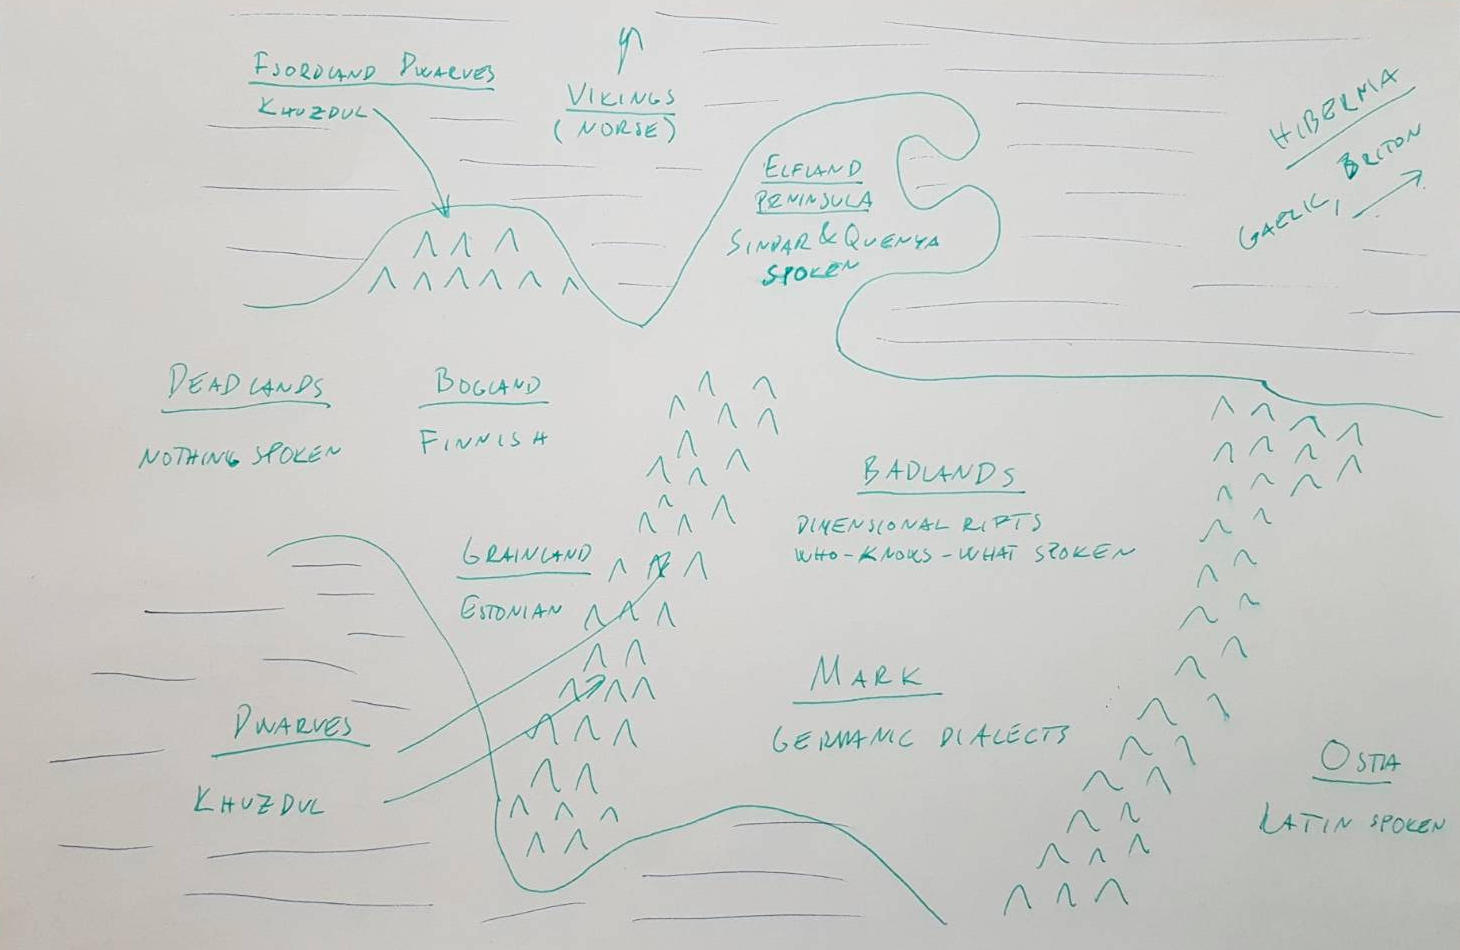
\includegraphics[width=\textwidth]{announ_cropped.png}
}

\frame{\frametitle{Alustavia periaatteita kielten lainaamiseen I}

Älä ota sitä mikä ei ole sinun -- ainakaan ilman lupaa.
\begin{itemize}
  \item Yksityisesti -- eli jos ei julkaise materiaalia missään -- voi toki
  käyttää (melkein) mitä vaan.
  \item On silti hyvä -- ja jopa hyödyllistä -- muistaa että tämän maailman
  kielten kylkiäisenä tulee yleensä kansa tai yhteisö, kulttuuri, fyysinen ja
  sosiaalinen ympäristö, ja historiaa. 
\end{itemize}
}


\frame{\frametitle{Alustavia periaatteita kielten lainaamiseen II}
Julkaistessa, pyydä lupa:
\begin{itemize}
  \item Keinotekoisista kielistä ainakaan osaa ei voit käyttää, koska lupaa ei
  saa.
  \item Lisäksi jos kielen yhteisö on jollain tapaa haavoittuvassa tai
  uhanalaisessa tilassa -- erityisesti kolonialisoinnin, vainoamisen tms vuoksi
  -- olisi hyvä pyytää lupaa kielen yhteisöltä. Ja se taas on yleensä paljon
  helpommin sanottu kuin tehty.
  \item Valtakielet ovat melko varmasti helpompi valinta, mutta on hyvä edelleen
  muistaa, että kielen ja murteen ja aksentin välinen ero on häilyvä. Ja jotkut
  murteet ja aksentit ovat oleellisesti sorrettujen vähemmistökielten asemassa.
\end{itemize}
}


\frame{\frametitle{Alustavia periaatteita kielten lainaamiseen III}
No mitä sitten lainata? Ainakin seuraavia on syytä miettiä:
\begin{itemize}
\item Edelliset kaksi diaa.
\item Halutaanko kielten olevan samalta aikakaudelta ja halutaanko kielen
vastaavan yhteiskunnan kehitysvaihetta (tähän palaataan kohta)?
\item Haittaako jos sekoitetaan luonnollisia ja keinotekoisia kieliä?
\item Mitä pidginejä ja creoleja ehkä tarvitaaan ja onko niille valmiita
vastineita? 
\item Millainen maailma on kyseessä ja mitä reunaehtoja se asettaa?
\end{itemize}
Ja\ldots
}

\frame{\frametitle{Alustavia periaatteita kielten lainaamiseen IV}
Miten kaikki tämä vuorovaikuttaa tarinan kanssa?
\begin{itemize}
\item Pitäisikö lainata vastaavasta kulttuurista vastaavaan? Vanhaa
pohjoisgermaanista kieltä puhuvat viikinginoloiset tyypit, latinaa vääntävä
maailman vallannut imperiumi?
\item Entäs ympäristö? Hyvä osa kielestä käsittelee säätä, ilmastoa,
kasvillisuutta, eläimiä, ja maastonmuotoja. Ja fyysinen ympäristö saattaa
vaikuttaa puheentuottoon.
\item Mitä eri kielet kertovat yhteisöjen historiallisista suhteista?
\item Entä jos haetaankin kontrastia tämän maailman tilanteeseen? Nykyaikaista
tekniikkaa käyttävät atsteekin puhujat maailmassa, jossa muut kansat ovat
teknisesti keskiajalla ja puhuvat modernia englantia?
\end{itemize}
}

\frame{\frametitle{Puut eivät haaraudu vain yhteen suuntaan ajassa}
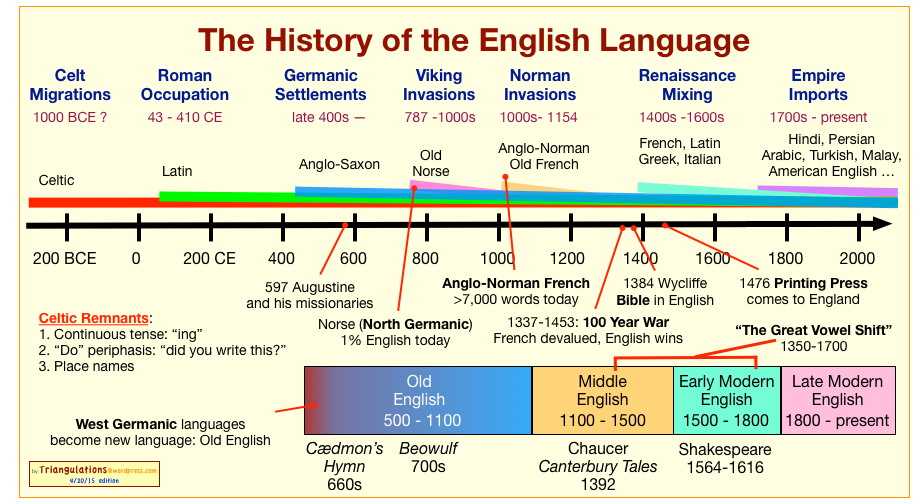
\includegraphics[width=\textwidth]{history_of_english5.png}
{\small Image from Triangulations blogger Sabio Lantz's blog post}
}

\frame{\frametitle{Varotaan haukkumasanoja ja muita ongelmia}
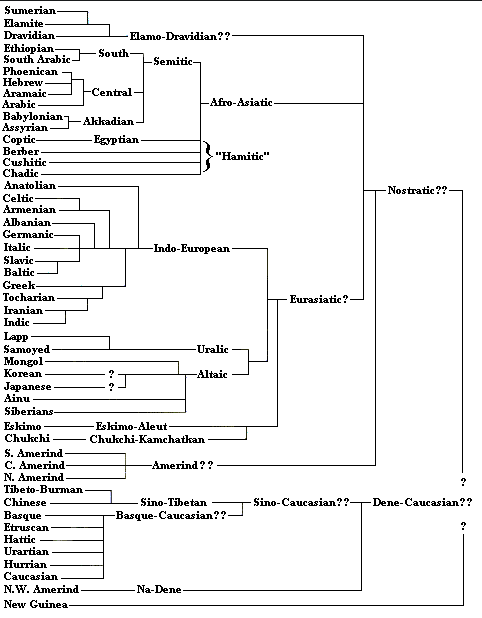
\includegraphics[width=.55\textwidth]{spot_the_pejorative_language_name_tree.png}
}

\frame{\frametitle{Kiitokset/Acknowledgements}

\begin{itemize}
  \item Again, the people who's ancestral land I have worked on.
  \item Sabio Lantz's blog post
  \url{https://triangulations.wordpress.com/2014/09/30/the-history-of-the-english-language-a-diagram/}
  \item Wikipedia is a lovely thing.
  \item All the good folk mentioned in passing and some that I've forgotten.
  \item Copyrighted work remains the property of the legal copyright holders.
  \item Last year's excellent participants.
  \item My work has been supported by a grant from Säätiöiden Post Doc pooli
  (they don't have an English name) / The Emil Aaltonen foundation.
  \end{itemize}
}

\frame{
\centering
\bf \Large 
\usebeamercolor[fg]{title}
Kiitokset myös teille!\\
~\\
Puhutaan!\\ 
~\\
Ja pidetään tauko hetken päästä.

}

\frame{
  \centering
  {
    \bf \Large 
    \usebeamercolor[fg]{title}
    Osa II\\
    ~\\
    Ideoita ((epä)todelliseen) puheeseen
    
    \vfill
  }
}

\frame{\frametitle{Mitä tehdään}


\begin{itemize}
    \item Joko vaan keskustellaan tai
    \item Työstetään pieniä tarinanaihioita:
    \begin{itemize}
      \item Työskennellään korkeintaan kuuden hengen ryhmissä.
      \item Esittelen ensin vähän ajatuksia lohikäärmeiden puheesta ja sitten
      muutaman muun tarinasiemenen.
      \item Työskennellään 20 minuuttia tarinoiden parissa kussakin ryhmässä.
      \item Jotta pysytään aikataulussa, kukin ryhmä työstää vain yhtä
      tarinasiementä.
      \item Lopuksi käydään tarinat pikaisesti läpi ja annan lyhyesti
      kannustavaa palautetta (n. 15 minuuttia yhteensä).
    \end{itemize}
    
\end{itemize}
}

\frame{\frametitle{Siemeniä}
Aiheen palat (olento ja genre):
\begin{itemize}
    \item Olento:
        \begin{enumerate}
        	\item humanoidi joka ei kuule eikä tuota ääntä
        	\item lohikäärme
        	\item tekoäly/demoni
        	\item lintu tai linnunkaltainen otus
        	\item hyönteinen tai hyönteisenkaltainen otus
        	\item jokin muu?
        \end{enumerate} 
   \item Genre:
        \begin{enumerate}
        	\item kasvutarina (ehkä fantasiaa, ehkä scifiä)
        	\item avaruusooppera
        	\item murhamysteeri
        	\item sankaritarina
        	\item historiallisehko fiktio
        	\item jokin muu?
        \end{enumerate}    
\end{itemize}
}

\frame{\frametitle{Mausteita}
\begin{itemize}
    \item Taikuus toimii puhumalla. Esimerkiksi maailman perusolemusta voi muokata puhuttavalla ohjelmointikielellä.
    \item Vihelletty tai rummutettu kieli.
    \item Laulu.
    \item Visuaalisest signaalit.
    \item Poikkeuksellinen äänentuotto: kurkkulaulutekniikat (tai niiltä
    kuulostaminen), Dune-leffan sardaukarien mörinä/korina. 
    \item Kääntämis- ja tulkkausongelmat.
    \item Mitä vaan keksitte.
\end{itemize}
}


% \frame{\frametitle{Some ideas to play around with}
% \begin{itemize}
%   \item If the world is magical, language can be too: 
%   \begin{itemize}
%     	\item Unholy, vowel rich language (cf. Moorcock): hääyöaie (i.e. you can
%     	do this with Finnish)
%     	\item "Guttural, evil language" was not a great idea to start with.
%   \end{itemize}  
%   \item Homophone words (think 'for' and 'four') and homonyms (see
%   \url{https://en.wikipedia.org/wiki/Homonym} for details) and other plays on words
%   can be part of a story ("Pedo mellon a minno.")
%   \begin{itemize}
%     \item Mix this with dialects and you can produce a pretty solidly confusing
%     situation.
%     \item Working these into game play may not be the easiest though.  
%   \end{itemize}
%   \item Whistled languages
%   \item Singing
% \end{itemize}
% }

\end{document}

